
\section{Learning Framework}
\label{sec:learning_framework}
Bagging and boosting are ensemble techniques very used in machine learning context. Due to the limited resources, we only tried the Bagging, but we can expect similar results with Boosting. 

Our final classifier is based on bagging of 5 weak models to predict the class of the object.\\
Each of the five weak classifier consists of two parts:
\begin{itemize}
    \item The first part, that we called "3D Backbone", or simply a Convolutional Neural Network (CNN) module; %\ac{CNN}
    \item followed by a fully connected multi-layer neural network.
\end{itemize}
\ \\
\textbf{\ref{sec:learning_framework}.1. 3D Backbone}

In the 3D Backbone, the Input/Output of various layers remain shaped in 3 dimension, preserving spatial relationship. This part can be split into 3 similar blocks, each block is composed by 3D layer as presented in the Fig.~\ref{fig:blockDiagram}

\begin{figure}[h]
\begin{center}
        \centering
        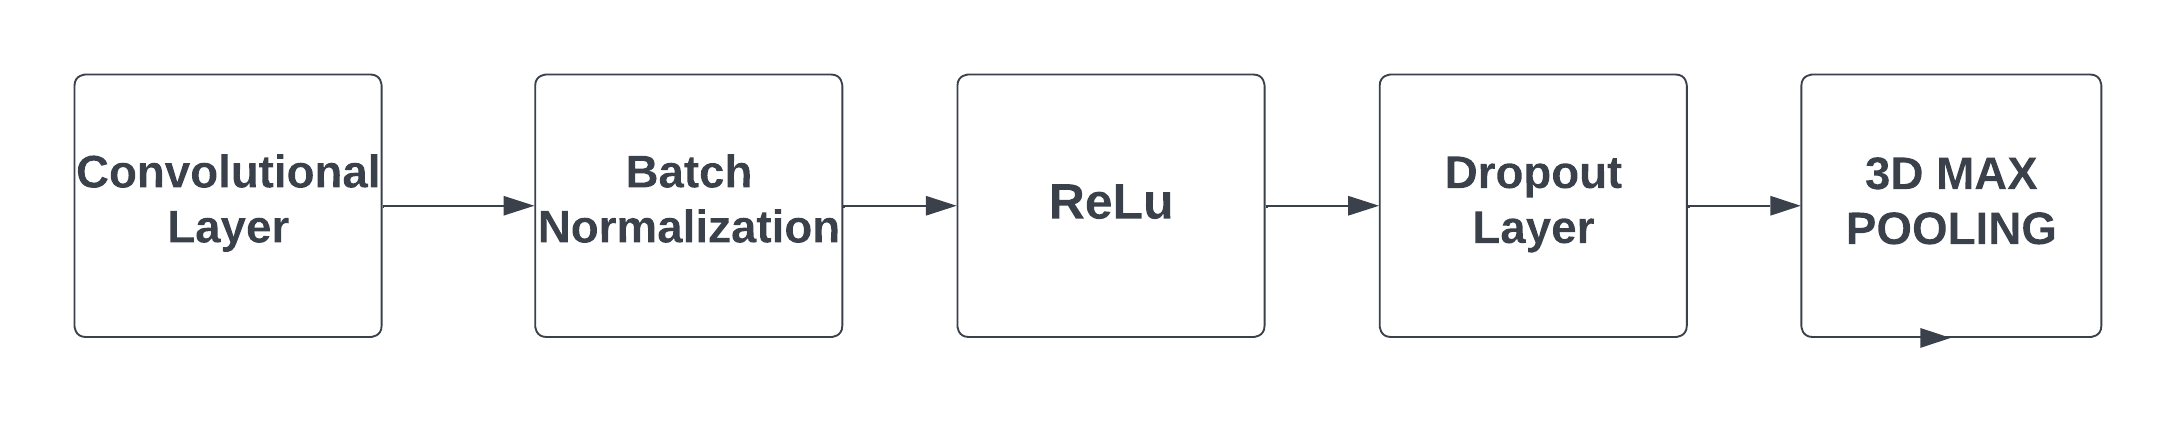
\includegraphics[width=0.5\textwidth]{resources/BlockDiagram.png}
        \caption{Single Layer of a 3D Backbone}
        \label{fig:blockDiagram}
    \end{center}
\end{figure}

The parameters for each of the block of the 3D backbone is reported in the Tab.~\ref{tab:conv-layers}.
We also test the Model with different learning rates and the one which seems to bring the best results was: Learning Rate = 1e-3.


\begin{table}[h]
\centering
\caption{Blocks of CNN 3D Backbone}
\label{tab:conv-layers}
\begin{tabular}{cccccc}
    \hline
    Block & Conv1 & Conv2 & Conv3 \\
    \hline
    Number of filters & 32 & 64 & 128 \\
    Kernel size & 3x3x3 & 3x3x3 & 3x3x3 \\
    Stride & 1 & 1 & 1   \\
    Padding & 1 & 1 & 1  \\
    Dropout ratio & 0.3 & 0.2 & 0.2  \\
    Max Pool Kernel & 2 & 2 & 2\\
    Max Pool Strides & 2 & 2 & 2\\
    Max Pool Paddings & 0 & 0 & 0\\
    \hline
\end{tabular}
\end{table}

\begin{table}[h]
    \centering
    \caption{Fully connected layers}
    \label{tab:fc-layers}
    \begin{tabular}{cccccc}
        \hline
        Layer & Fc1 & Fc2  \\
        \hline
        Number of Outputs & 128 & 10 \\
        Dropout ratio & 0.4 & 0.0   \\
        
        \hline
    \end{tabular}
\end{table}

\ \\
\textbf{\ref{sec:learning_framework}.1. FC network}

The second part of the weak model is composed by 2 fully connected layers. As is common for multi-class classification tasks, the output activation function in the final layer of our models is softmax.
\begin{equation}
    \sigma(\mathbf{z})_j = \frac{e^{z_j}}{\sum_{k=1}^{K}e^{z_k}}
\end{equation}
% \[
% \sigma(\mathbf{z})_j = \frac{e^{z_j}}{\sum_{k=1}^{K}e^{z_k}}
% \]
where
\begin{itemize}
    \item \textbf{z} represent the vector given in input to the softmax function
    \item z\textsubscript{j} the j\textsubscript{th} element of z
    \item \textbf{K} is the number of classes
\end{itemize}

Since the Convolutional backbone maintains the 3-dimensional shape of the object, in order to make the models make its prediction we flattened the output of backbone in a 1 dimension array, and given in input to the first Fully connected layer, which parameters are reported in the Tab.~\ref{tab:fc-layers}. The softmax function requires that the final output of the models has the number of outputs equal to the number of classes, and so it is.

The loss used for our models is the Cross-entropy loss, which is a common choice for multi-class classification tasks. It measures the dissimilarity between the predicted probability distribution by the softmax function and the true probability distribution of the target variable.
The Cross-entropy loss function has the following equations:
\begin{equation}
 L(p, y) = - (y * log(p) + (1 - y) * log(1 - p)) 
\end{equation}

Cross-entropy loss is calculated for each example in the training data, and the average loss over all examples is used as the final loss value.
We decided to run each of our model for 100 epochs, this choice was made to explore and capture the behavior of the models during the training phase, but how we will see in the next chapter, the models converges with less than 100 epochs.

The final result of the ensembled model is obtained by merging the prediction of all models, we tested two method to take the final prediction:
\begin{itemize}
    \item \textbf{Summing the Probabilities:} We sum the results of the softmax function from all the weak classifiers. The class with the highest sum of probabilities is then chosen as the final prediction. 
    \item \textbf{Voting:} In this method, each model in the ensemble makes its prediction, the final result is taken as the most voted class. 
\end{itemize}
    We tested both methodologies and in the end we decided to use the first approach, "sum the probabilities", for mainly two reasons, the first is that thanks to Softmax function we can explicit a sort of "belief" of correctness from a model, and we want to use this information for the final prediction, and the second reason is that having only 5 models it implies that the voting system may too easily end up in a tie, which may lead to uncertain results, e.g. 2 votes for class "bed", 2 votes for class "table", and 1 vote for class "bathtub". 
    
In the next chapter we will visualize and comment the results obtained
